\chapter{The GLLAMM for dichotomous outcomes} \label{chap:framework}

The Generalized Linear Latent and Mixed Model (GLLAMM) is a framework that unifies a wide range of latent variable models. Developed by Rabe-Hesketh and colleagues \cite{Rabe_et_al_2004a, Rabe_et_al_2004b, Rabe_et_al_2004c, Skrondal_et_al_2004a, Rabe_et_al_2012}, the method was motivated by the need of a Multilevel Structural Equation Model (MSEM) that accommodated for unbalanced data, noncontinuous responses and cross-level effects among latent variables. The authors focused its development mainly from the frequentist perspective, however, they offered a general guidance on implementing the model under the bayesian framework (see \citet{Skrondal_et_al_2004a}).


\section{Model motivation} \label{sect:motivation}

Consider a large standardized assessment composed of three sub-test designed to evaluate the reading comprehension, mathematical reasoning, and pedagogical knowledge of teachers; where each sub-test has several dichotomously scored items. 

Focusing on the first sub-test, the items were designed to measure only one of the three hierarchically nested sub-dimensions of reading comprehension: literal, inferential, and reflective abilities. Furthermore, it is assumed the three sub-dimensions are all that is needed to measure the reading comprehension ability, effectively making this scale the highest level latent variable in the model, similar to a hierarchical Confirmatory Factor Analysis (CFA). Finally, the items were bundled in groups of five to a common text or passage, i.e. testlets, that provided the stimulus over which the individual is assessed. Figure \ref{fig:design} shows the path diagram of the hypothesized dimensional structure, for the hierarchical cross-classified IRT model corresponding with the instrument.

\begin{figure}[h] \label{fig:design}
	\centering
	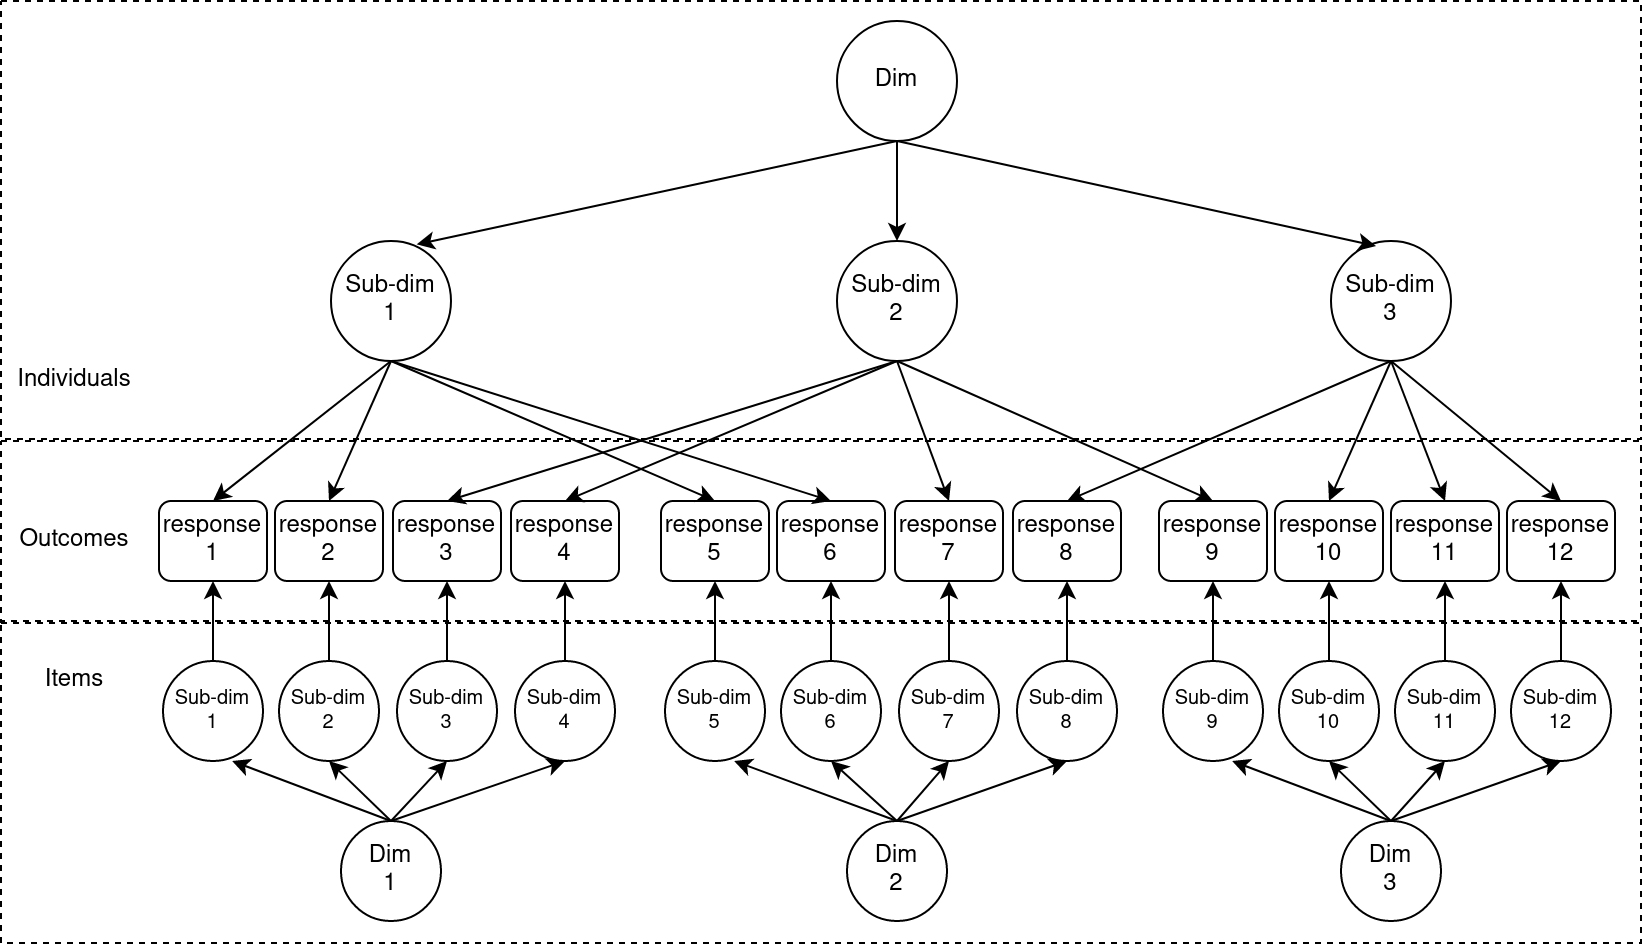
\includegraphics[width=0.85\textwidth]{instrument_design.png}
	\caption[Path diagram of the dimensional structure for a hierarchical cross-classified IRT model.]%
	{Path diagram of the dimensional structure for a hierarchical cross-classified IRT model. Squares represent dichotomous manifest variables, and circles represent latent variables. The figure is based on a reduced set of items, while the errors and scales of the latent variables are not represented. Different sub-dimensions at the individuals block represent the literal, inferential and reflective abilities, while at the items blocks represent the items' difficulties. The dimensions at the individuals block represent the reading comprehension ability, while at the items block represent the multiple testlets.}
\end{figure}

With the purpose of providing an easier motivation of the model, we will not consider yet the cluster effects; however, later in the presentation we will show how easy is to introduce them in the model. Just for future reference, under this example, one expects to observe clustering effects, because individuals from different regions did not have the same educational opportunities, effectively causing differences among them at a regional level.


\section{Model definition} \label{sect:definition}

Following \citet{Rabe_et_al_2004a, Rabe_et_al_2004b}, we continue defining the GLLAMM in two parts: (i) the response model, and (ii) the latent structure.

In case the reader is interested in outcomes different than the dichotomous case, refer to Appendix \ref{appA1:links}.

\subsection{Response model} \label{s_sect:response}

Conditional on the regression parameters $\pmb{\beta}$, loadings $\pmb{\Lambda}$, explanatory and latent variables ($\mathbf{X},  \pmb{\Theta}$), the response model can be represented by a Generalized Linear Model (GLM) \cite{Nelder_et_al_1972, Nelder_et_al_1989} with a distributional and a systematic part. The latter composed of a linear predictor and a link function.

For the distributional part, the dichotomous items $y_{jkd}$ are modeled at the first level by a Bernoulli probability mass function $f(\cdot)$, in the following form:
\begin{equation} \label{eq:distributional}
	\begin{split}
		f \left( y_{jkd}=1 \; | \; \mathbf{X}, \pmb{\beta}, \pmb{\Lambda}, \pmb{\Theta} \right) &= \pi_{jkd}^{n} (1 - \pi_{jkd})^{1-n}
	\end{split}
\end{equation}

\noindent where $n$ denotes the endorsement of the item in the Bernoulli trial. On the other hand, in the systematic part, the probability of endorsing the item $\pi_{jkd}$ is linked to a linear predictor $v_{jkd}$ through an inverse-link function $h(\cdot)$, in the following form:
\begin{equation} \label{eq:systematic}
	\begin{split}
		P\left[ y_{jkd}=1 \; | \; \mathbf{X}, \pmb{\beta}, \pmb{\Lambda}, \pmb{\Theta} \right] &= \pi_{jkd} = h( \tau_{k} + v_{jkd} )
	\end{split}	
\end{equation}

\noindent where $\tau_{k}$ is $k$'th item threshold, assumed to be zero for the binary case \cite{Rabe_et_al_2004a}. Furthermore, the inverse-link function can be defined in three ways:	
\begin{equation} \label{eq:response_dich1}
	h(x) = 
	\begin{cases}
		exp(x)[1 + exp(x)]^{-1} \\
		%
		\Phi(x)  \\
		%
		exp(-exp(x))
	\end{cases}
\end{equation}

\noindent corresponding to the logistic, standard normal $\Phi(x)$, and Gumbel (extreme value type I) cumulative distributions, respectively. It is usual to report the last in terms of link functions $g(\cdot) = h^{-1}(\cdot)$. In that case, the link functions corresponds to the well known logit, probit and complementary log-log, respectively. Finally, the linear predictor is defined by:
\begin{equation} \label{eq:linear_predictor1}
	\begin{split}
		v_{jkd} &= \sum_{p=1}^{P} x_{jp} \beta_{p} + \sum_{m=2}^{M+1} \sum_{k=1}^{K_{(m)}} \eta_{k}^{(m)} \alpha_{k}^{(m)} + \sum_{l=2}^{L+1} \sum_{d=1}^{D_{(l)}} \theta_{jd}^{(l)} \lambda_{d}^{(l)}
	\end{split}
\end{equation}

\noindent where individuals are indexed by $j = 1, \dots, J$, and $J$ represents the total number of individuals in the sample. $\beta_{p}$ denotes regression parameter for the $x_{jp}$ explanatory variable with $p=1,\dots, P$, and $P$ denoting the total number of explanatory variables. $\eta_{k}^{(m)}$ is the $k$th item latent dimension at level $m$ with loading $\alpha_{k}^{(m)}$, where $k= 1, \dots, K_{(m)}$, $K_{(m)}$ denotes the number of dimensions at level $m=2,\dots, M+1$, and $M$ represents the number of levels in the items block. $\theta_{jd}^{(l)}$ denotes the individual's $d$th latent dimension at level $l$ with loading $\lambda_{d}^{(l)}$, where $d=1, \dots, D_{(l)}$, $D_{(l)}$ represents the number of dimensions at level $l=2, \dots, L+1$, and $L$ denotes the number of levels observed in the individuals block. Using figure \ref{fig:design} as a reference, we have $P=0$, as we do not have explanatory variables; $M=2$ levels in the items bock, where $K_{2}=12$ corresponding to the items difficulties, and $K_{3}=3$ corresponding to the testlets effects; and $L=2$ levels in the individuals block, with $D_{2}=3$ corresponding to the literal, inferential and reflective abilities, and $D_{3}=1$ corresponding to the reading comprehension latent variable.

Equation (\ref{eq:linear_predictor1}) can be re-written in matrix form in the following way:
\begin{equation} \label{eq:linear_predictor2}
	\begin{split}
		v_{jkd} &= \mathbf{X}_{j} \pmb{\beta} + \sum_{m=2}^{M+1} \pmb{\eta}^{(m)} \pmb{\alpha}^{(m)} \mathbf{A}_{j}^{(m)} + \sum_{l=2}^{L+1} \pmb{\theta}_{j}^{(l)} \pmb{\lambda}^{(l)} \mathbf{B}_{j}^{(l)}
	\end{split}
\end{equation}

\noindent where $\mathbf{X}_{j}$ represents the individual's design matrix of explanatory variables that maps the parameter vector $\pmb{\beta}$ to the linear predictor. Moreover, $\pmb{\eta}^{(m)} = [ \eta_{1}^{(m)}, \dots, \eta_{K_{(m)}}^{(m)} ]^{T}$, and  $\pmb{\alpha}^{(m)} = [ \alpha_{1}^{(m)}, \dots, \alpha_{K_{(m)}}^{(m)} ]^{T}$ are the vectors of the item's latent dimensions with corresponding loadings at level $m$, mapped by a block matrix $\mathbf{A}_{j}^{(m)}$. Similarly, $\pmb{\theta}_{j}^{(l)} = [ \theta_{j1}^{(l)}, \dots, \theta_{jD_{(l)}}^{(l)} ]^{T}$, and  $\pmb{\lambda}^{(l)} = [ \lambda_{1}^{(l)}, \dots, \lambda_{D_{(l)}}^{(l)} ]^{T}$ are the vectors of the individuals's latent dimensions with corresponding loadings at level $l$, mapped by a block matrix $\mathbf{B}_{j}^{(l)}$.

Notice the model departs from the traditional multivariate framework for formulating structural models, i.e. a wide data format, where the subject’s repeated outcomes are stored in a single row, with multiple response vectors and explanatory variables appended column-wise to the outcome data; and adopts a univariate approach, i.e. a long data format, where the subject’s repeated outcomes are stored in a single ``stacked" response vector with as many rows as there are repeated measurements, and explanatory variables appended column-wise to the outcome data, distinguished from each other, by a design block matrix. 

Finally, as it was declared at the beginning of the section, we will use $\mathbf{X} = [ \mathbf{X}_{1}^{T}, \dots, \mathbf{X}_{J}^{T} ]^{T}$ to represent the ``stacked" design matrix of explanatory variables for all individuals. Furthermore, $\pmb{\Lambda} = [ \pmb{\alpha}^{(2)T}, \dots, \pmb{\alpha}^{(M+1)T}, \pmb{\lambda}^{(1)T}, \dots, \pmb{\lambda}^{(L+1)T} ]^{T}$ will represent the ``stacked" vector of loadings, and $\pmb{\Theta} = [ \pmb{\eta}^{(2)T}, \dots, \pmb{\eta}^{(M+1)T}, \pmb{\theta}^{(2)T}, \dots, \pmb{\theta}^{(L+1)T} ]^{T}$ as the ``stacked" vectors of dimensions and sub-dimensions.



\subsubsection{Cluster effects} \label{ss_sect:clusters}

Considering the previous, we can see that modeling clustering is as easier as to add more random effects to the linear predictor defined in equation (\ref{eq:linear_predictor1}), in the following form:
\begin{equation} \label{eq:linear_predictor3}
	\begin{split}
		v_{jkdc} &= v_{jkd} + \sum_{c=1}^{C} \delta_{c}  \\
		%
		&= v_{jkd} + \pmb{\delta} \mathbf{Z}_{j}
	\end{split}
\end{equation}
\noindent where $c=1, \dots, C$, which denotes the number of clusters, $v_{jkd}$ is defined as in equation (\ref{eq:linear_predictor1}), and $\mathbf{Z_{j}}$ is a design block matrix.
	


\subsection{Latent structure} \label{s_sect:struct}
The structural model for the latent variables presents the following form:
\begin{equation} \label{eq:structural_model}
	\def\sss{\scriptstyle}
	\setstackgap{L}{12pt}
	\def\stacktype{L}
	\pmb{\Theta} = \stackunder{\pmb{\Psi}}{\sss (S \times S)} \stackunder{\pmb{\Theta}}{\sss (S \times 1)} + \stackunder{\pmb{\Gamma}}{\sss (S \times Q)} \stackunder{\mathbf{W}}{\sss (Q \times 1)} + \stackunder{\pmb{\zeta}}{\sss (S \times 1)}
\end{equation}

\noindent where $S=K+D$, $K = \sum_{m} K_{m}$, and $D = \sum_{l} D_{l}$. Furthermore, $\pmb{\Psi}$ and $\pmb{\Gamma}$ are parameter matrices that map the relationship between the latent variables $\pmb{\Theta}$, and the ``stacked" vector of covariates $\mathbf{W}$, respectively; while $\pmb{\zeta}$ is a vector of errors or disturbances. It is important to indicate that $\mathbf{W}$ considers a different set of covariates from $\mathbf{X}$, as we hypothesize they explain the variability in the latent variables at different levels (see chapter \ref{chap:estimation} and \ref{chap:application} for the implementation in the context of a real dataset).

Notice equation (\ref{eq:structural_model}) resembles to single-level Structural Equation Models (SEM), however, the main difference in the GLLAMM representation is that the latent variables may vary at different levels. 

Additionally, considering that $\pmb{\Theta}$ has no feedback effects, is permuted, and sorted according to the levels of interest, then $\pmb{\Psi}$ will be a strictly upper triangular matrix. In this regard, (i) the absence of feedback loops imply the method deals with non-recursive models, i.e. none of the latent variables are specified as both causes and effects of each other \cite{Kline_2012}; and (ii) the strictly upper triangular structure reveals the GLLAMM does not allow latent variables to be regressed on lower level latent or observed variables, implying the method deals with reflective latent variables, i.e. the higher level latent variables are thought to be the cause of the lower level latent or manifest variables \cite{Beaujean_2014}. For a more detailed explanation on the topic refer to \citet{Edwards_et_al_2000}.
